\chapter{Analyse fonctionnelle}

\section{Interview}

Après notre interview avec notre encadrant Ali Mansour, nous avons réalisé un tableau des spécifications suivantes:

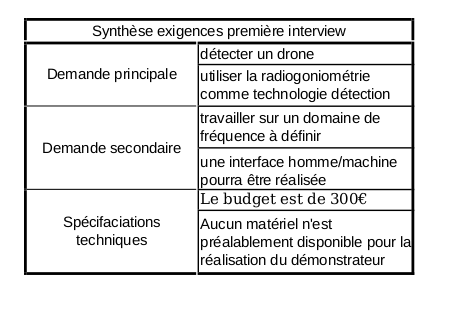
\includegraphics[width=0.8\textwidth]{interview}


\section{Tableau des spécifications}
En prenant en compte les recommandations de notre encadrant, et les recherches que nous avons réalisées, nous avons établi les contraintes et les spécifications suivantes:

%\includegraphics[width=\textwidth]{tableauSpe}
\includepdf{./images/tableauSpe.pdf}

%Compte tenu des recherches que nous avons réalisées, nous avons établi l'étude fonctionnelle suivante.

%De la synthèse de ce tableau découle le diagramme Pieuvre et les SADT suivant.

\section{Diagramme pieuvre}
~\\
~\\
~\\
~\\
~\\
~\\
\hspace{-2cm}
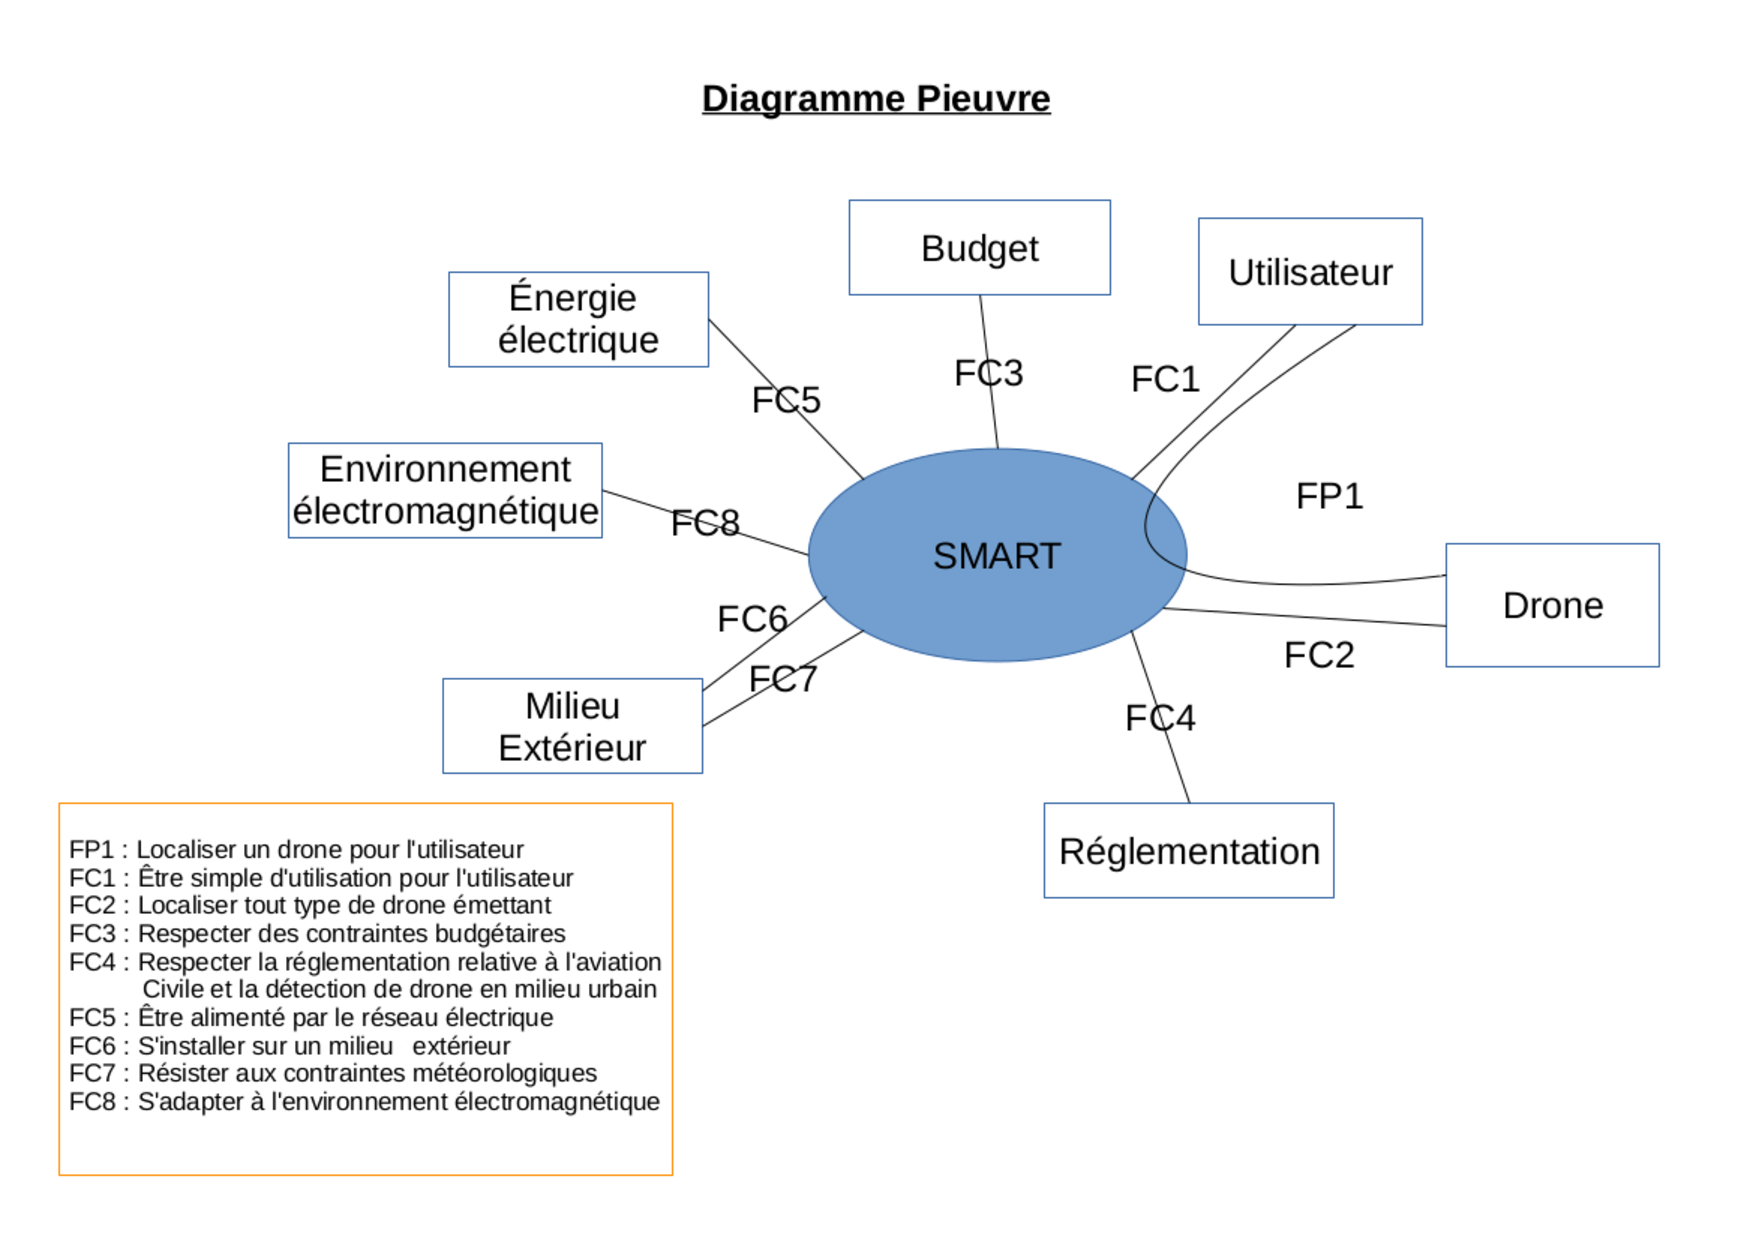
\includegraphics[width=1.18\textwidth]{Diagramme_pieuvre.pdf}
\captionof{figure}{Diagramme pieuvre}



\section{SADT}

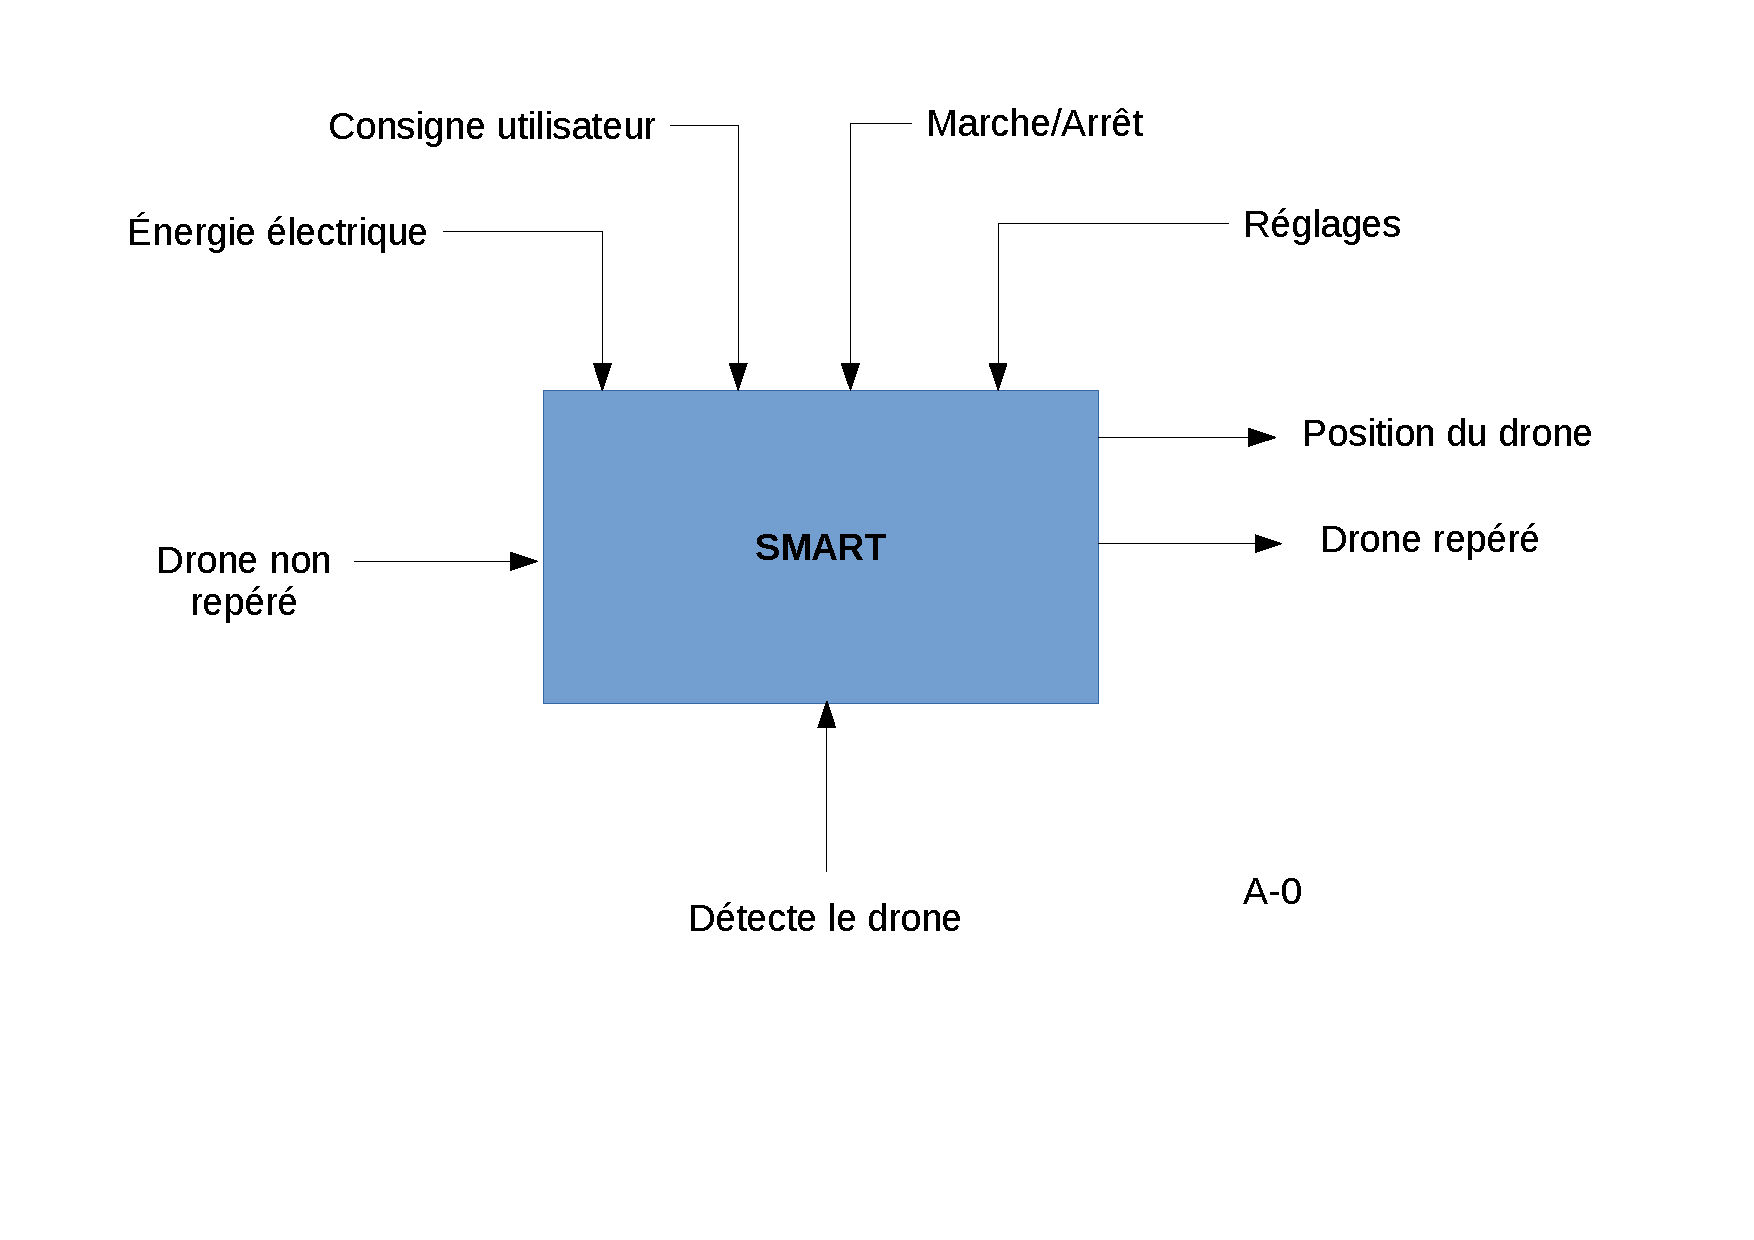
\includegraphics[width=\textwidth]{SADT_A-0.pdf}
\captionof{figure}{SADT A-0}
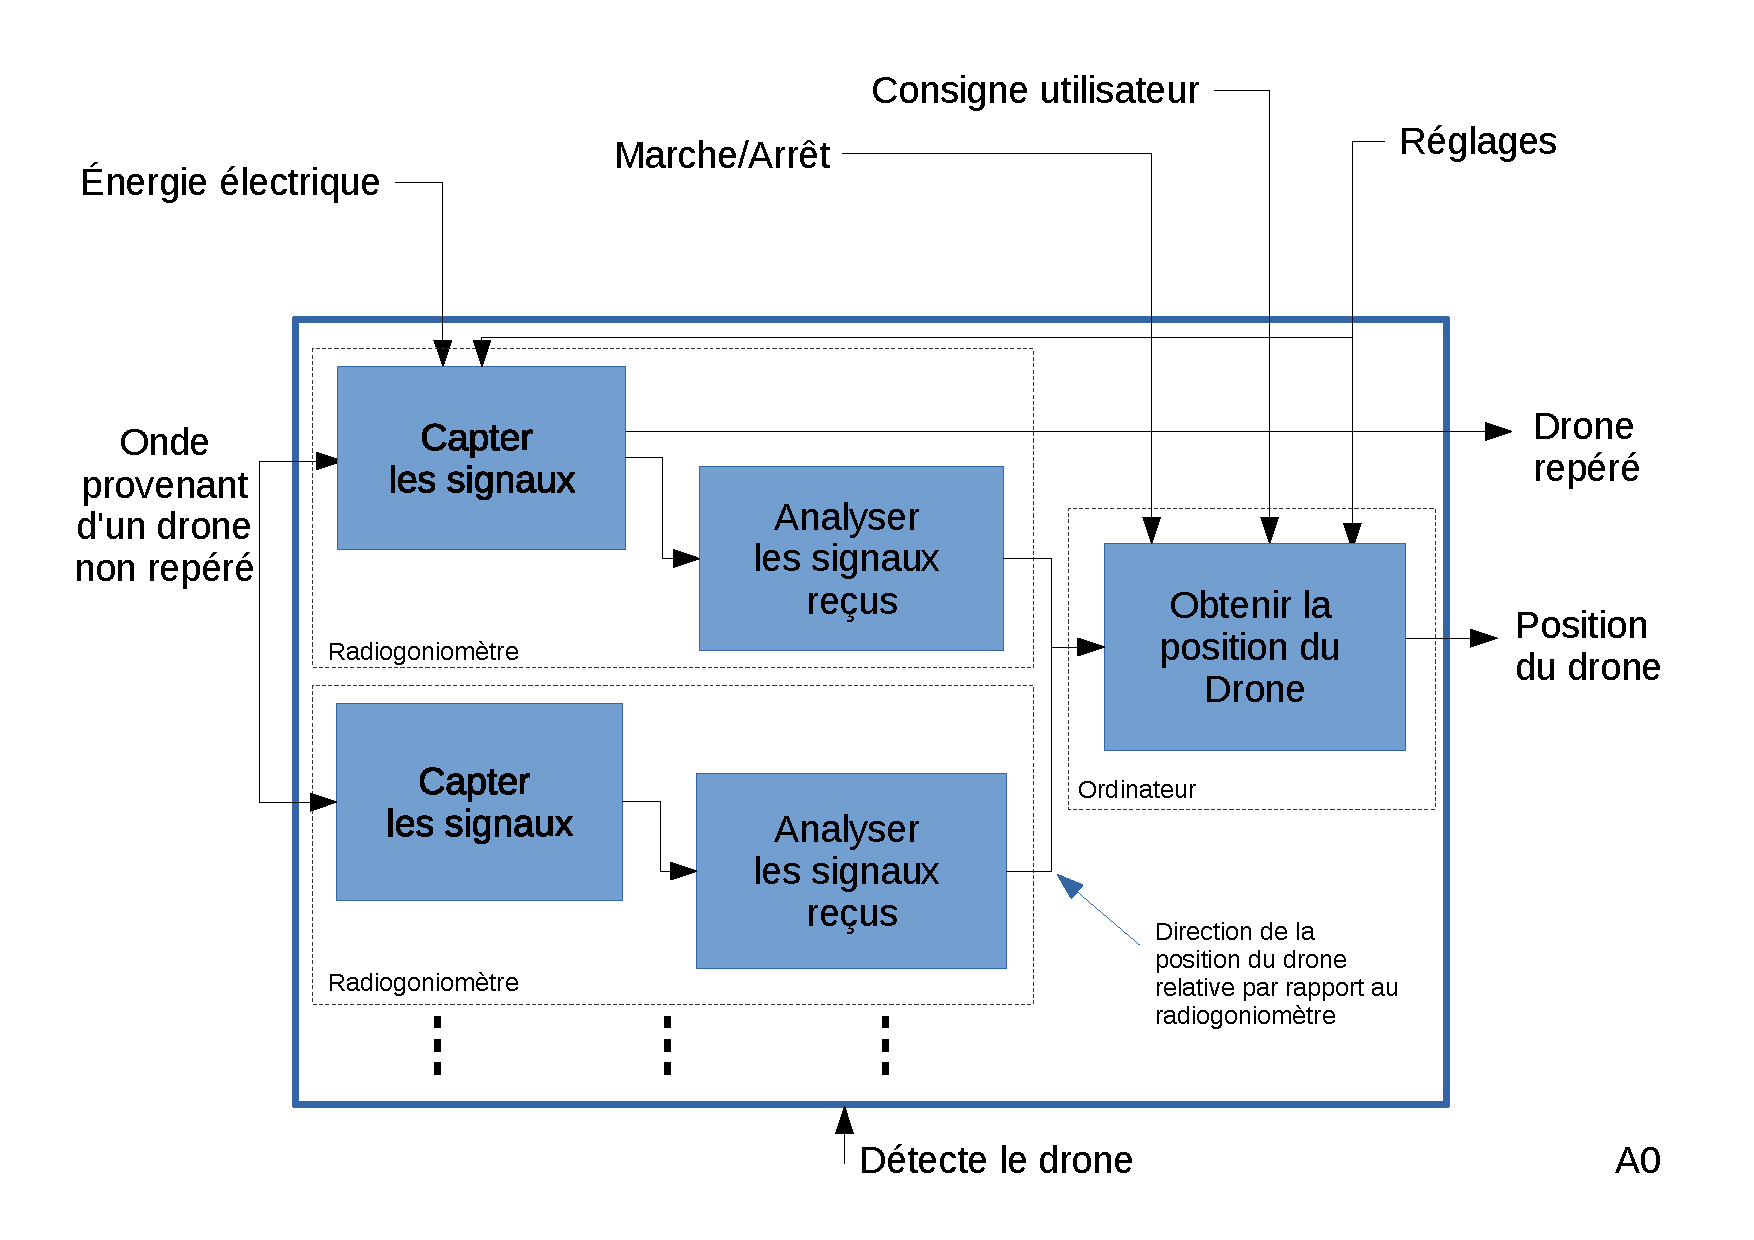
\includegraphics[width=\textwidth]{SADT_A0.pdf}
\captionof{figure}{SADT A0}

\newpage
\parindent=15pt

Comme on peut le voir sur le SADT A0, nous avons découpé notre objectif en trois parties.

Dans un premier temps il faut capter les signaux. Pour cela il faut réaliser un balayage sur le radiogoniomètre pour détecter les bons signaux.

Ensuite, il faut analyser les signaux reçus pour s'assurer que nous sommes bien en présence d'un drone.

Enfin, il faut récupérer les données des radiogoniomètres pour déterminer la position du drone.


\section{FAST}

\hspace{-1.5cm}
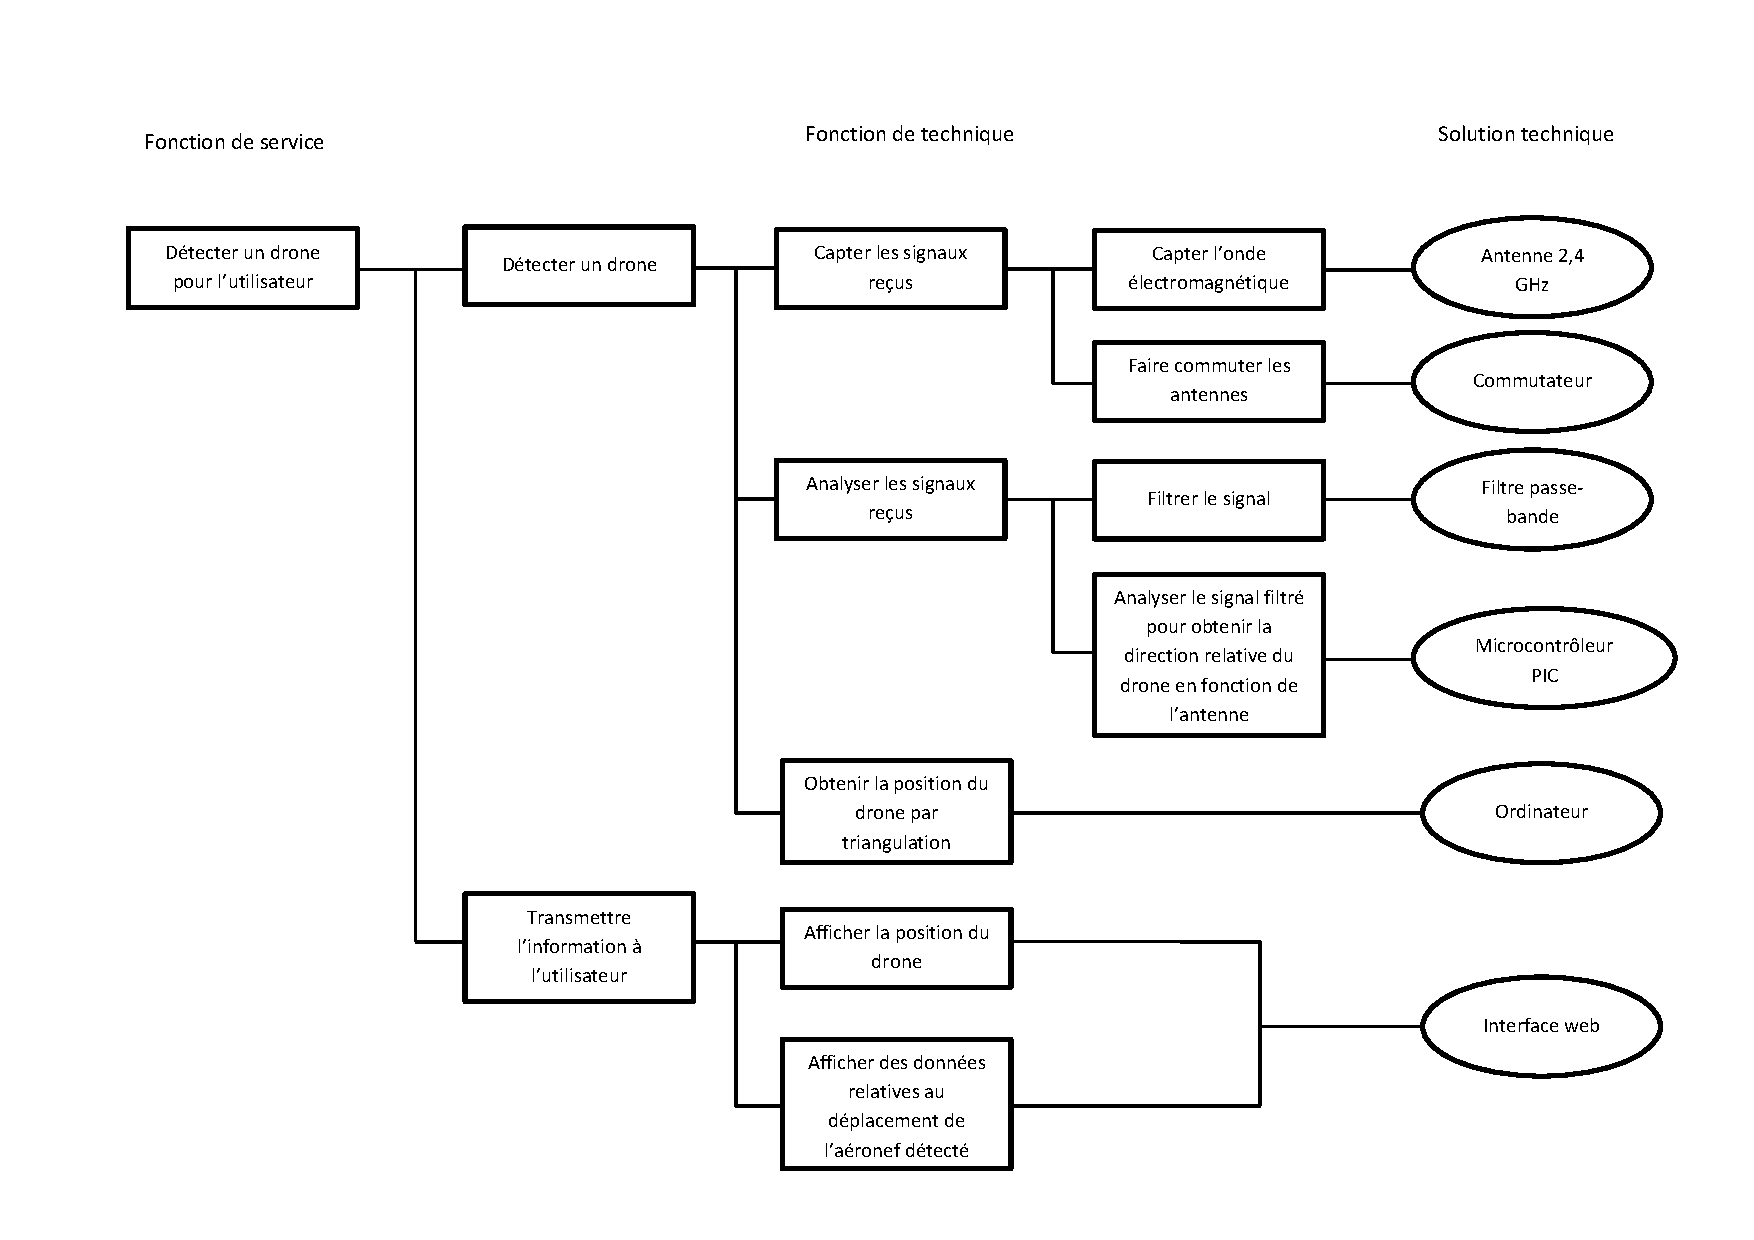
\includegraphics[width=1.2\textwidth]{FAST.pdf}
\captionof{figure}{Diagramme FAST}


\section{Diagramme 3 axes}

\hspace{-1.5cm}
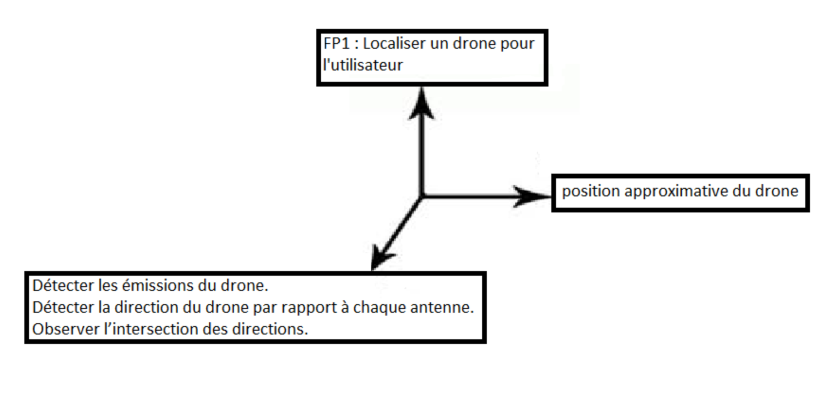
\includegraphics[width=1.2\textwidth]{3axes.pdf}
\captionof{figure}{Diagramme 3 axes}
\parindent=15pt
~\\

Le diagramme 3 axes ci-dessus présente les étapes clefs du traitement du problème. En effet, la
détection d’un drone nécessite de repérer une perturbation dans la bande de fréquence que l’on écoute,
de détecter la direction de laquelle elle provient et enfin de regrouper les données pour, à partir des
directions, obtenir la position.

\section{Fonctionnement de notre système}

Nous avons donc imaginé positionner plusieurs radiogoniomètres, chaque appareil indiquerait la direction du drone par rapport à sa position. Chacun d'eux serait connecté à un ordinateur central qui analyserai chacune des positions données par les radiogoniomètres et en déduirait la position du drone dans l'espace.

~\\

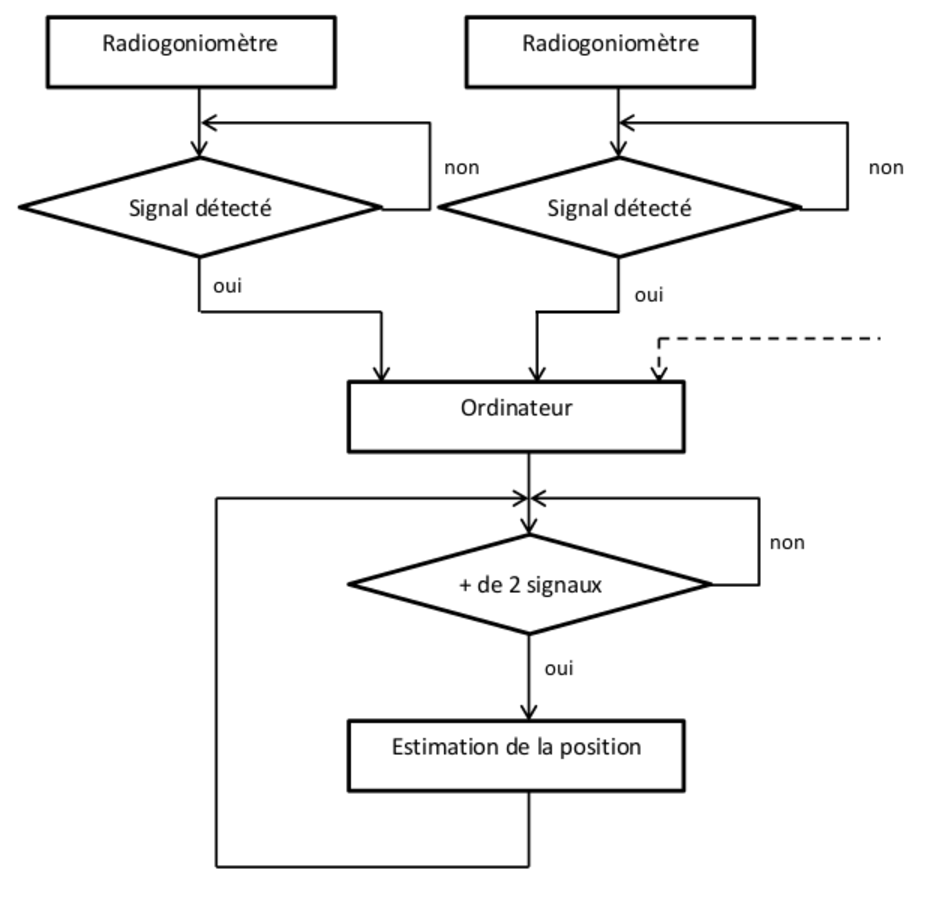
\includegraphics[width=0.8\textwidth]{SMART_logic}
\captionof{figure}{Schéma Logique du système}
\parindent=15pt



%%% Local Variables: 
%%% mode: latex
%%% TeX-master: "rapport_analyse"
%%% End: 
